\documentclass[a4paper,11pt]{article}

% Package imports - reordered and fixed for local compilation
\usepackage[T1]{fontenc}
\usepackage[utf8]{inputenc}
\usepackage{latexsym}
\usepackage{xcolor}
\usepackage{float}
\usepackage{ragged2e}
\usepackage[empty]{fullpage}
\usepackage{wrapfig}
\usepackage{tabularx}
\usepackage{titlesec}
\usepackage{geometry}
\usepackage{marvosym}
\usepackage{verbatim}
\usepackage{enumitem}
\usepackage{fancyhdr}
\usepackage{multicol}
\usepackage{graphicx}
\usepackage{microtype}
\usepackage{array} % Required for vertical centering in tables

% Font packages - using more compatible options
\usepackage{lmodern} % Latin Modern fonts (replacement for cfr-lm)
\usepackage{fontawesome} % FontAwesome icons (more compatible than fontawesome5)

% Hyperref should be loaded last
\usepackage[hidelinks]{hyperref}

% tcolorbox - using basic version for better compatibility
\usepackage{tcolorbox}

% Color definitions
\definecolor{darkblue}{RGB}{0,0,139}

% Page layout
\geometry{left=1.4cm, top=0.8cm, right=1.2cm, bottom=1cm}
\setlength{\multicolsep}{0pt} 
\pagestyle{fancy}
\fancyhf{} % clear all header and footer fields
\fancyfoot{}
\renewcommand{\headrulewidth}{0pt}
\renewcommand{\footrulewidth}{0pt}
\setlength{\footskip}{4.08pt}

% Hyperlink setup
\hypersetup{
    colorlinks=true,
    linkcolor=darkblue,
    filecolor=darkblue,
    urlcolor=darkblue,
}

% Custom box settings - simplified for better compatibility
\tcbset{
    frame code={},
    center title,
    left=0pt,
    right=0pt,
    top=0pt,
    bottom=0pt,
    colback=gray!20,
    colframe=white,
    width=\dimexpr\textwidth\relax,
    enlarge left by=-2mm,
    boxsep=4pt,
    arc=0pt,outer arc=0pt,
}

% URL style
\urlstyle{same}

% Text alignment
\raggedright
\setlength{\tabcolsep}{0in}

% Section formatting
\titleformat{\section}{
  \vspace{-4pt}\scshape\raggedright\large\bfseries
}{}{0em}{}[\color{black}\titlerule \vspace{-7pt}]

% Custom commands
\newcommand{\resumeItem}[2]{
  \item{
    \textbf{#1}{\hspace{0.5mm}#2 \vspace{-0.5mm}}
  }
}

% New command for different font sizes and indentation in bullet points
\newcommand{\resumeItemMain}[1]{
  \item #1
}

\newcommand{\resumeItemSub}[1]{
  \item[] \hspace{0.05mm} $\diamond$ {\small #1}
}

\newcommand{\resumeItemSubSub}[1]{
  \item[] \hspace{0.1mm} $\ast$ {\footnotesize #1}
}

\newcommand{\resumePOR}[3]{
\vspace{0.5mm}\item
    \begin{tabular*}{0.97\textwidth}[t]{l@{\extracolsep{\fill}}r}
        \textbf{#1}\hspace{0.3mm}#2 & \textit{\small{#3}} 
    \end{tabular*}
    \vspace{-2mm}
}

% Modified resumeSubheading to move dates to right margin
\newcommand{\resumeSubheading}[4]{
\vspace{0.5mm}\item
    \begin{tabular*}{0.98\textwidth}[t]{l@{\extracolsep{\fill}}r}
        \textbf{#1} & \textit{\footnotesize{#4}} \\
        \textit{\footnotesize{#3}} & \footnotesize{#2} \\
    \end{tabular*}
    \vspace{-2.4mm}
}

\newcommand{\resumeProject}[4]{
\vspace{0.5mm}\item
    \begin{tabular*}{0.98\textwidth}[t]{l@{\extracolsep{\fill}}r}
        \textbf{#1} & \textit{\footnotesize{#3}} \\
        \footnotesize{\textit{#2}} & \footnotesize{#4}
    \end{tabular*}
    \vspace{-2.4mm}
}

\newcommand{\resumeSubItem}[2]{\resumeItem{#1}{#2}\vspace{-4pt}}

% Bullet point symbols for different levels
\renewcommand{\labelitemi}{\raisebox{0.2ex}{\large$\bullet$}}
\renewcommand{\labelitemii}{$\vcenter{\hbox{\scriptsize$\circ$}}$}
\renewcommand{\labelitemiii}{$\vcenter{\hbox{\tiny$\diamond$}}$}
\renewcommand{\labelitemiv}{$\vcenter{\hbox{\scriptsize$\ast$}}$}

% List environment commands - simplified to avoid nesting issues
\newcommand{\resumeSubHeadingListStart}{\begin{itemize}[leftmargin=*,labelsep=0.1mm]}
\newcommand{\resumeHeadingSkillStart}{\begin{itemize}[leftmargin=*,itemsep=1.7mm, rightmargin=2ex]}
\newcommand{\resumeItemListStart}{\begin{itemize}[leftmargin=*,labelsep=1mm,itemsep=0.5mm]}

\newcommand{\resumeSubHeadingListEnd}{\end{itemize}\vspace{2mm}}
\newcommand{\resumeHeadingSkillEnd}{\end{itemize}\vspace{-2mm}}
\newcommand{\resumeItemListEnd}{\end{itemize}\vspace{-2mm}}

\newcommand{\cvsection}[1]{%
\vspace{2mm}
\begin{tcolorbox}
    \textbf{\large #1}
\end{tcolorbox}
    \vspace{-4mm}
}

\newcolumntype{L}{>{\raggedright\arraybackslash}X}%
\newcolumntype{R}{>{\raggedleft\arraybackslash}X}%
\newcolumntype{C}{>{\centering\arraybackslash}X}%

% Commands for icon sizing and positioning - simplified
\newcommand{\socialicon}[1]{\raisebox{-0.05em}{\resizebox{!}{1em}{#1}}}
\newcommand{\ieeeicon}[1]{\raisebox{-0.3em}{\resizebox{!}{1.3em}{#1}}}

% Font options - using more compatible font commands
\newcommand{\headerfonti}{\sffamily} % Sans serif
\newcommand{\headerfontii}{\rmfamily} % Roman (serif)
\newcommand{\headerfontiii}{\ttfamily} % Typewriter

% Define personal information
\newcommand{\name}{Ikhsan Moekhtar} % Your Name
\newcommand{\course}{Bachelor of Engineering} % Your Course
\newcommand{\roll}{XXXXXX} % Your Roll No.
\newcommand{\phone}{81261289573} % Your Phone Number
\newcommand{\emaila}{ikhsanmoekhtar890098@gmail.com} % Email 1
\newcommand{\emailb}{officialemail@nitp.ac.in} % Email 2
\newcommand{\github}{IkhsanMoekhtar} % Github
%\newcommand{\website}{https://syahrul-fathoni.vercel.app} % Website
\newcommand{\linkedin}{ikhsan-moekhtar-7501b3252} % LinkedIn

\begin{document}
\sloppy
\rmfamily % Using standard roman family instead of cmr

%----------HEADING-----------------
\parbox{2.35cm}{%
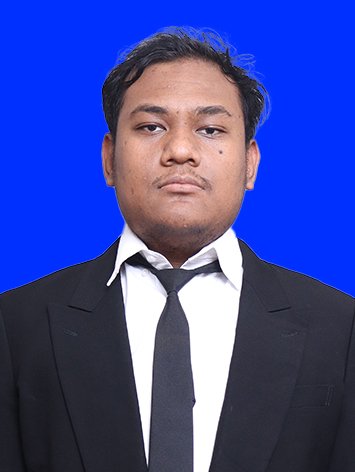
\includegraphics[width=2cm,clip]{2.jpg}
}
\parbox{\dimexpr\linewidth-2.8cm\relax}{
\begin{tabularx}{\linewidth}{L r}
  \textbf{\LARGE \name} & +62-\phone \\
  \course & \href{mailto:\emailb}{\emaila} \\
  Computer Engineering & \href{https://www.linkedin.com/in/\linkedin}{linkedin.com/in/\linkedin} \\
  Institut Teknologi Sepuluh Nopember, Surabaya
  & \href{https://github.com/\github}{github.com/\github} \\
  %& \href{https://syahrul-fathoni.vercel.app}{syahrul-portfolio-web}
\end{tabularx}
}
\vspace{-2mm}

\section{\textbf{Education}}
\vspace{1mm}
\setlength{\tabcolsep}{5pt}
\begin{tabularx}{\textwidth}{|>{\centering\arraybackslash}X|>{\centering\arraybackslash}p{8cm}|>{\centering\arraybackslash}p{3cm}|>{\centering\arraybackslash}p{2.5cm}|}
  \hline
  \textbf{Degree} & \textbf{Institute} & \textbf{Current CGPA} & \textbf{Year} \\
  \hline
  S.T., Teknik Komputer & Institut Teknologi Sepuluh Nopember, Surabaya & 3.33/4.0 & Aug 2025 \\ 
  \hline
\end{tabularx}
\vspace{-4mm}

\section{\textbf{Skills}}
\vspace{-0.4mm}
\resumeHeadingSkillStart
    \resumeSubItem{Full-Stack Development}{: Python, JavaScript, Node.js, Express.js, Flask, API, PostgreSQL, HTML/CSS, flutter, kotlin, Firebase}
    \resumeSubItem{AI \& IoT Systems}{: PyTorch, LSTM, ESP32, Arduino, C++, C}
    \resumeSubItem{DevOps \& Cloud}{: Git, Vercel, Apache Kafka}
\resumeHeadingSkillEnd
\vspace{-2mm}

\section{\textbf{Work Experiences}}
\vspace{-0.4mm}
\resumeSubHeadingListStart

\resumeSubheading
    {Bangkit Academy led by Google, Tokopedia, Gojek, \& Traveloka}{Surabaya, Indonesia}
    {Mobile Development Cohort}{Feb 2024 - July 2024}
    \resumeItemListStart
        \resumeItemMain{\textbf{Capstone Project - EdukaOne: Chatbot to Assist Student in Learning}}
        \resumeItemSub{Led a team of seven to develop \textbf{EdukaOne}, a mobile application designed to help students learn in a structured way and provide learning materials using AI Chatbot.}

        \resumeItemMain{\textbf{Mobile Application Development with Kotlin}}
        \resumeItemSub{Created a cross-platform mobile application using Kotlin, integrating RESTful APIs for real-time data access and user authentication.}
    \resumeItemListEnd

\resumeSubHeadingListEnd
\vspace{-6mm}

\section{\textbf{Individual Projects}}
\vspace{-0.4mm}
\resumeSubHeadingListStart

\resumeProject{\parbox{0.8\linewidth}{PitchPlus+: AI-Powered Futsal Match Analysis.}}
{Tools: Python, Express.js, Node.js, CSS, HTML, React.js}
{Sep 2024 - Dec 2024}{}
\resumeItemListStart
    \resumeItemMain{Developed an AI-powered futsal match analysis system that provides statistics and insights, enhancing player performance and game strategy.}
    \resumeItemMain{Implemented a web application using Node.js for backend development and React.js for the frontend, enabling users to upload match videos and receive detailed analyses through a user-friendly interface.}
\resumeItemListEnd

\resumeProject
    {SISTEM VISUALISASI REKAM MEDIS BERBASIS DATA ECG PASIEN}
    {Tools: PostgreSQL, Python, Flask, HTML, Flutter, Dart}
    {May 2025 - July 2025}
    {{}[\href{https://github.com/IkhsanMoekhtar/test_ecgreader}
    {\textcolor{darkblue}{\faGithub}}]}
\resumeItemListStart
    \resumeItemMain{Implemented a comprehensive data visualization system for ECG recordings, enabling healthcare professionals to analyze patient data effectively.}
    \resumeItemMain{Create a system that allows ECG raw data or .SCP type data to be stored and visualized in  mobile application using Flutter framework.}
\resumeItemListEnd
\resumeSubHeadingListEnd
\vspace{-8mm}

\section{\textbf{Campus Organization Experiences}}
\vspace{-0.4mm}
\resumeSubHeadingListStart
\resumeSubheading
    {MAGE (Multimedia And Game Event) 9}{Surabaya, Indonesia}
    {Logistics Coordinator}{Feb 2023 - Mar 2024}
    \resumeItemListStart
        \resumeItemMain{Authorized to organize logistics in running the event, preparing the venue and necessary items for Indonesia's premier technology competition catering to all high school students among Indonesia.}
    \resumeItemListEnd
\resumeSubHeadingListEnd
\vspace{-6mm}

\section{\textbf{Certifications}}
\vspace{-0.4mm}
\resumeSubHeadingListStart
    \resumePOR
    {Independent Study Program - Bangkit Academy}
    {, \href{https://drive.google.com/file/d/1rzM9lUdXGklJ5xKt6RPXNg5od7ZojOkw/view?usp=sharing}{Program-Certificate}}
    {Feb 2024 - June 2024}
    \resumePOR
    {Android Application Fundamental by Dicoding}
    {, \href{https://drive.google.com/file/d/1btvdw1g6GOZVza8Tbb_Vl2fyNNSZfwMh/view?usp=sharing}{Course}}
    {April 2024}
    \resumePOR
    {Programming With Kotlin By Dicoding}
    {, \href{https://drive.google.com/file/d/1m7H74zXfivIhVCQJl3cOw2oXn39I5kyF/view?usp=sharing}{Course}}
    {Feb 2024}
\resumeSubHeadingListEnd
\end{document}